\documentclass[11pt,twocolumn]{article}
\usepackage{caption}
\usepackage{anysize}
\usepackage{fancyhdr}
\usepackage{graphicx}
\usepackage{subcaption}
\usepackage{color}
\usepackage{balance}
\usepackage{lipsum}
\usepackage{multirow}
\usepackage{multicol}
\usepackage{booktabs}
\usepackage{pgfplots}
\usepackage{tabulary}

\marginsize{.75in}{.75in}{.75in}{1in}
\pagestyle{fancy}
\rhead{\today}
\lhead{
\includegraphics[height=2.0cm]{../logo.jpg}}
\rfoot{\thepage}
\cfoot{}
\renewcommand{\headrulewidth}{0pt} %removes line from fancy header
\renewcommand{\thispagestyle}[1]{} %placers header and footer on first page 
\renewcommand{\abstractname}{Summary}
\setlength{\columnsep}{25pt}
\date{}
\title{Laboratory Gasification Memo\\Enthalpy Experiments \vspace{-6ex}}

\begin{document}

\twocolumn[
  \begin{@twocolumnfalse}
    \maketitle
    \begin{abstract}
    
In order to obtain an understanding if the main driving force for conversion of biomass to syngas is driven by residence time or heat transfer limitations, an experimental matrix was designed to examine different levels of space time and the maximum possible enthalpy change of the reactants.

    \end{abstract}
  \end{@twocolumnfalse}
]

\section*{Experimental Methods}

\subsection*{Design of Experiment}

It was desired to create a two factorial matrix with a center point with the two axes representing maximum residence time (t$_{res,max}$) and maximum enthalpy change ($\Delta$H$_{max}$).  The matrix can be seen in Figure \ref{factorial}.  Partial pressure of steam and partial pressure of CO$_2$ was held constant for these experiments at 7 psi and 30 psi, respectively.  These values were chosen because a large number of previous gasification experiments had partial pressures of CO$_2$ and H$_2$O near these values.  

Because of the large number of possible set points in the laboratory gasifier system that would effect both the space time and maximum enthalpy simultaneously, it would have been difficult to manually design this experimental matrix.  To aid in the design, a large number of potential gasifier experiments were simulated using Sundrop Fuels' gasifier analysis software suite.  First, a flow rate of CO$_2$ was randomly assigned using a uniform distribution with a minimum possible flow rate of 3 SLPM and a maximum flow rate of 6.6 SLPM.  The partial pressure of CO$_2$ was set at 7 psi, and the appropriate flow rate of steam to lead to a partial pressure of 30 psi was found with Equation \ref{eq_steam}.

The flow rate of Argon was set at 2 SLPM for all experiments.  Biomass flow rate was randomized uniformly between 2 lbs/hr and 4 lbs/hr.  The total flow rate of entrainment gas was set to be 6 SLPM for every 1 lb/hr of biomass, which was found to be a good minimum entrainment flow rate in previous experiments using the brush feeder.  The remainder of the entrainment gas which isn't CO$_2$ is nitrogen.

Steam temperature is set at 500 $^\circ$C, and makeup nitrogen is uniformly randomized between 0 and 20 SLPM.  The total pressure is found using the partial pressure of steam and the total flow rate of gas into the system (Equation \ref{pressure}).  The maximum residence time and the maximum enthalpy change were calculated for each simulated run using Sundrop Fuel's gasifier analysis software.  Experiments which could not be run due to system limitations were removed from the potential runs, and enthalpy and maximum residence time targets were chosen to maximize the change in each measure.  Set points for all experiments are outlined in Appendix \ref{app_experiments}.

\begin{equation}
	\dot{n}_{H_2O} = \dot{n}_{CO_2} \times \frac{P_{H_2O}}{P_{CO_2}}
	\label{eq_steam}
\end{equation}

\begin{equation}
	P_{tot} = P_{H_2O} \times \frac{\dot{n}_{tot}}{\dot{n}_{H_2O}}
	\label{pressure}
\end{equation}

\begin{figure}
\centering
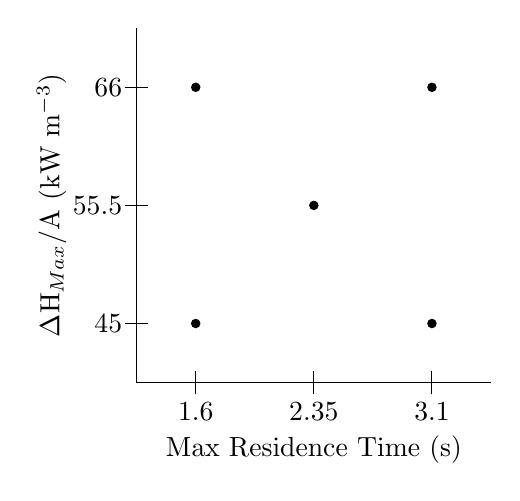
\begin{tikzpicture}[scale = 1.5]
	\draw (0,0) -- (3,0);
	\draw (0,0) -- (0,3);
	\draw (0.5,-0.1) -- (0.5,0.1) node[below = 8pt] {1.6}
		(1.5,-0.1) -- (1.5,0.1) node[below = 8pt] {2.35} node[below = 20pt]{Max Residence Time (s)}
		(2.5,-0.1) -- (2.5,0.1) node[below = 8pt] {3.1}
		(-0.1,0.5) -- (0.1,0.5) node[left = 6pt] {45}
		(-0.1,1.5) -- (0.1,1.5) node[left = 6pt] {55.5} node[xshift = -35pt, rotate = 90]{$\Delta$H$_{Max}$/A (kW m$^{-3}$)}
		(-0.1,2.5) -- (0.1,2.5) node[left = 6pt] {66};
	\filldraw [black] (0.5,0.5) circle (1pt)
		(2.5,0.5) circle (1pt)
		(1.5,1.5) circle (1pt)
		(0.5,2.5) circle (1pt)
		(2.5,2.5) circle (1pt);
\end{tikzpicture}
\caption{Two factorial experimental matrix used to vary maximum residence time and maximum $\Delta$H between experiments.}
\label{factorial}
\end{figure}

\subsection*{Calculations}

Two measures of carbon conversion are discussed in this memo.  The first is the fraction of carbon in the biomass which is converted to either CO or CO$_2$, as these are the two species which are the precursor to synthetic liquid products in the planned commercial process.  This measure is refered to as ``carbon yield", although it has been referred to in the past as ``good conversion," and is given in Equation \ref{eq_c_yield}.

\begin{equation}
	Y_{CO+CO_2} = \frac{\dot{n}_{CO,out}+\dot{n}_{CO_2,out} - \dot{n}_{CO_2,in}}{\dot{n}_{C_{biomass},in}}
	\label{eq_c_yield}
\end{equation}

The second measure is ``carbon release", which has been referred to in the past as ``total conversion."  This is calculated using Equation \ref{eq_c_release} and is a representation of the fraction of carbon in the biomass which is converted to any gaseous specie.

\begin{equation}
	X_{C} = \frac{\dot{n}_{C_{gas},out}- \dot{n}_{CO_2,in}}{\dot{n}_{C_{biomass},in}}
	\label{eq_c_release}
\end{equation}

\section*{Results and Discussion}

\subsection*{Carbon Yield}

Carbon yield results are plotted in Figures \ref{maxrt_vs_cyield}, \ref{minrt_vs_cyield}, \ref{dh_vs_cyield_maxrt}, and \ref{dh_vs_cyield_minrt}.  ANOVA results are given in Table \ref{anova_cyield}, and factors which had a statistically significant effect on carbon yield are highlighted in red.  At 1350 $^\circ$C, minimum residence time was not statistically significant while $\Delta H_{Max}$/A was.  Both minimum residence time and $\Delta H_{Max}$/A were statistically signficant at 1450 $^\circ$C.  However, as shown in the aforementioned plots, higher residence times led to lower carbon yields, if there was an effect.  Since this is the reverse of what would be expected, it's possible that the effect did not exist, or another factor was correlated with the changing residence times that is causing the difference in calculated carbon yields.  Further tests may be held in the future holding different factors constant to see if the effect seen goes away at 1450 $^\circ$C.

\begin{table}
	\centering
	\caption{ANOVA results on effects of designed experimental campaign for carbon yield.}
	\begin{tabular}{r c c}
		\toprule
		\multicolumn{1}{c}{\multirow{2}{*}{Effect}}		& 	\multicolumn{2}{c}{Prob \textless F	}	\\
		{}								&	1350 $^\circ$C					&	1450 $^\circ$C			\\
		\midrule
		t$_{res,min}$						&	0.1845						&	\textcolor{red}{0.0059}	\\
		$\Delta H_{Max}$/A					&	\textcolor{red}{\textless 0.0001}	&	\textcolor{red}{0.0002}	\\
		t$_{res,min}\times \Delta H_{Max}$/A	&	0.5060						&	0.9646				\\
		\bottomrule
	\end{tabular}
	\label{anova_cyield}
\end{table}

\begin{figure*}
\centering
% Maximum Residence Time vs X_good Colored by dH_max %
	\begin{tikzpicture}
	\begin{axis} [scale = .9,
		title =  1450 $^\circ$C,
		xlabel = Maximum Residence Time (s), 
		ylabel= Carbon Yield,
		yticklabel style = {/pgf/number format/.cd,fixed zerofill}, 
		xticklabel style = {/pgf/number format/.cd,fixed zerofill,precision=1}, 
		colorbar horizontal, 
		colorbar style = {
			at={(1.15,-.35)},anchor=north,
			xticklabel style = {/pgf/number format/.cd,fixed zerofill,precision=0}, 
			xlabel=$\frac{\Delta H Max}{A} (\frac{kW}{m^2})$, 
			xlabel style = {yshift = 1.7cm},
			point meta min = 45}
]
	\addplot[
		scatter, 
		only marks, 
		scatter src = explicit,] 
		table [
			col sep = comma,
			x = space_time_avg, 
			y = X_good_avg, 
			meta = dH/A]  
	{enthalpy_runs_1450.csv};
	\end{axis}
	\begin{axis} [scale = .9, at={(7.5cm,0)},
		title =  1350 $^\circ$C,
		xlabel = Maximum Residence Time (s), 
		yticklabel style = {/pgf/number format/.cd,fixed zerofill}, 
		xticklabel style = {/pgf/number format/.cd,fixed zerofill,precision=1}]
	\addplot[
		scatter, 
		only marks, 
		scatter src = explicit,] 
		table [
			col sep = comma,
			x = space_time_avg, 
			y = X_good_avg, 
			meta = dH/A]  
	{enthalpy_runs_1350.csv};
	\end{axis}

	\end{tikzpicture}
	\caption{Blah blah blah blah SDPFOICJPFOIJD}
	\label{maxrt_vs_cyield}
\end{figure*}




\begin{figure*}
\centering
% Minimum Residence Time vs X_good Colored by dH_max %
	\begin{tikzpicture}
	\begin{axis} [scale = .9,
		title =  1450 $^\circ$C,
		xlabel = Minimum Residence Time (s), 
		ylabel= Carbon Yield,
		yticklabel style = {/pgf/number format/.cd,fixed zerofill}, 
		xticklabel style = {/pgf/number format/.cd,fixed zerofill,precision=2}, 
		colorbar horizontal, 
		colorbar style = {
			at={(1.15,-.35)},anchor=north,
			xticklabel style = {/pgf/number format/.cd,fixed zerofill,precision=0}, 
			xlabel=$\frac{\Delta H Max}{A} (\frac{kW}{m^2})$, 
			xlabel style = {yshift = 1.7cm},
			point meta min = 45}
]
	\addplot[
		scatter, 
		only marks, 
		scatter src = explicit,] 
		table [
			col sep = comma,
			x = tau_min, 
			y = X_good_avg, 
			meta = dH/A]  
	{enthalpy_runs_1450.csv};
	\end{axis}
	\begin{axis} [scale = .9, at={(7.5cm,0)},
		title =  1350 $^\circ$C,
		xlabel = Minimum Residence Time (s), 
		yticklabel style = {/pgf/number format/.cd,fixed zerofill}, 
		xticklabel style = {/pgf/number format/.cd,fixed zerofill,precision=2}, 
		xtick = {.3,.4,.5,.6}
]
	\addplot[
		scatter, 
		only marks, 
		scatter src = explicit,] 
		table [
			col sep = comma,
			x = tau_min, 
			y = X_good_avg, 
			meta = dH/A]  
	{enthalpy_runs_1350.csv};
	\end{axis}
	\end{tikzpicture}
	\caption{Blah blah blah blah SDPFOICJPFOIJD}
	\label{minrt_vs_cyield}
\end{figure*}



\begin{figure*}
\centering
% dH/A vs X_good Colored by space_time %
	\begin{tikzpicture}
	\begin{axis} [scale = .9,
		title =  1450 $^\circ$C,
		xlabel = $\frac{\Delta H Max}{A} (\frac{kW}{m^2})$, 
		ylabel= Carbon Yield,
		yticklabel style = {/pgf/number format/.cd,fixed zerofill}, 
		xticklabel style = {/pgf/number format/.cd,fixed zerofill,precision=1}, 
		colorbar horizontal, 
		colorbar style = {
			at={(1.15,-.35)},anchor=north,
			xticklabel style = {/pgf/number format/.cd,fixed zerofill,precision=1}, 
			xlabel=Maximum Residence Time (s), 
			xlabel style = {yshift = 1.7cm},
			xtick = {1.5,2.3,3.0},
			point meta min = 1.4
}
]
	\addplot[
		scatter, 
		only marks, 
		scatter src = explicit,] 
		table [
			col sep = comma,
			x = dH/A, 
			y = X_good_avg, 
			meta = space_time_avg]  
	{enthalpy_runs_1450.csv};
	\end{axis}
	\begin{axis} [scale = .9, at={(7.5cm,0)},
		title =  1350 $^\circ$C,
		xlabel = $\frac{\Delta H Max}{A} (\frac{kW}{m^2})$, 
		yticklabel style = {/pgf/number format/.cd,fixed zerofill}, 
		xticklabel style = {/pgf/number format/.cd,fixed zerofill,precision=1}, 
]
	\addplot[
		scatter, 
		only marks, 
		scatter src = explicit,] 
		table [
			col sep = comma,
			x = dH/A, 
			y = X_good_avg, 
			meta = space_time_avg]  
	{enthalpy_runs_1350.csv};
	\end{axis}
	\end{tikzpicture}
	\caption{Blah blah blah blah SDPFOICJPFOIJD}
	\label{dh_vs_cyield_maxrt}
\end{figure*}


\begin{figure*}
\centering
% dH/A vs X_good Colored by minimum residence time %
	\begin{tikzpicture}
	\begin{axis} [scale = .9,
		title =  1450 $^\circ$C,
		xlabel = $\frac{\Delta H Max}{A} (\frac{kW}{m^2})$, 
		ylabel= Carbon Yield,
		yticklabel style = {/pgf/number format/.cd,fixed zerofill}, 
		xticklabel style = {/pgf/number format/.cd,fixed zerofill,precision=0}, 
		colorbar horizontal, 
		colorbar style = {
			at={(1.15,-.35)},anchor=north,
			xticklabel style = {/pgf/number format/.cd,fixed zerofill,precision=2}, 
			xlabel=Minimum Residence Time (s), 
			xlabel style = {yshift = 1.7cm}
}
]
	\addplot[
		scatter, 
		only marks, 
		scatter src = explicit,] 
		table [
			col sep = comma,
			x = dH/A, 
			y = X_good_avg, 
			meta = tau_min]  
	{enthalpy_runs_1450.csv};
	\end{axis}
	\begin{axis} [scale = .9, at={(7.5cm,0)},
		title =  1350 $^\circ$C,
		xlabel = $\frac{\Delta H Max}{A} (\frac{kW}{m^2})$, 
		yticklabel style = {/pgf/number format/.cd,fixed zerofill}, 
		xticklabel style = {/pgf/number format/.cd,fixed zerofill,precision=1}, 
]
	\addplot[
		scatter, 
		only marks, 
		scatter src = explicit,] 
		table [
			col sep = comma,
			x = dH/A, 
			y = X_good_avg, 
			meta = tau_min]  
	{enthalpy_runs_1350.csv};
	\end{axis}
	\end{tikzpicture}
	\caption{Blah blah blah blah SDPFOICJPFOIJD}
	\label{dh_vs_cyield_minrt}
\end{figure*}



\subsection*{Carbon Release}

Carbon release results are plotted in Figures \ref{maxrt_vs_crel}, \ref{minrt_vs_crel}, \ref{dh_vs_crel_maxrt}, and \ref{dh_vs_crel_minrt}.  Results from ANOVA reflected what was seen in carbon yield measurements.  The total maximum enthalpy load was a significant factor in the carbon release at both 1450 $^\circ$C and 1350 $^\circ$C.  Again, while minimum residence time was statistically significant at 1450 $^\circ$C, longer residence times actually gave lower conversions.  Since this result is the opposite of what should be expected for longer residence times, further tests may be completed in the future to see if some other factor correlated with the changing residence times was causing the apparent dependency of conversion on residence time.

\begin{table}
	\centering
	\caption{ANOVA results on effects of designed experimental campaign for carbon release.}
	\begin{tabular}{r c c}
		\toprule
		\multicolumn{1}{c}{\multirow{2}{*}{Effect}}		& 	\multicolumn{2}{c}{Prob \textless F	}	\\
		{}								&	1350 $^\circ$C			&	1450 $^\circ$C			\\
		\midrule
		t$_{res,min}$						&	0.1175				&	\textcolor{red}{0.0017}	\\
		$\Delta H_{Max}$/A					&	\textcolor{red}{0.0005}	&	\textcolor{red}{0.0002}	\\
		t$_{res,min}\times \Delta H_{Max}$/A	&	0.8289				&	0.7615				\\
		\bottomrule
	\end{tabular}
	\label{}
\end{table}

\begin{figure*}
\centering
% Maximum Residence Time vs X_tot Colored by dH_max %
	\begin{tikzpicture}
	\begin{axis} [scale = .9,
		title =  1450 $^\circ$C,
		xlabel = Maximum Residence Time (s), 
		ylabel= Carbon Release,
		yticklabel style = {/pgf/number format/.cd,fixed zerofill}, 
		xticklabel style = {/pgf/number format/.cd,fixed zerofill,precision=1}, 
		colorbar horizontal, 
		colorbar style = {
			at={(1.15,-.35)},anchor=north,
			xticklabel style = {/pgf/number format/.cd,fixed zerofill,precision=0}, 
			xlabel=$\frac{\Delta H Max}{A} (\frac{kW}{m^2})$, 
			xlabel style = {yshift = 1.7cm},
			point meta min = 45}
]
	\addplot[
		scatter, 
		only marks, 
		scatter src = explicit,] 
		table [
			col sep = comma,
			x = space_time_avg, 
			y = X_tot_avg, 
			meta = dH/A]  
	{enthalpy_runs_1450.csv};
	\end{axis}
	\begin{axis} [scale = .9, at={(7.5cm,0)},
		title =  1350 $^\circ$C,
		xlabel = Maximum Residence Time (s), 
		yticklabel style = {/pgf/number format/.cd,fixed zerofill}, 
		xticklabel style = {/pgf/number format/.cd,fixed zerofill,precision=1}]
	\addplot[
		scatter, 
		only marks, 
		scatter src = explicit,] 
		table [
			col sep = comma,
			x = space_time_avg, 
			y = X_tot_avg, 
			meta = dH/A]  
	{enthalpy_runs_1350.csv};
	\end{axis}

	\end{tikzpicture}
	\caption{Blah blah blah blah SDPFOICJPFOIJD}
	\label{maxrt_vs_crel}
\end{figure*}




\begin{figure*}
\centering
% Minimum Residence Time vs X_tot Colored by dH_max %
	\begin{tikzpicture}
	\begin{axis} [scale = .9,
		title =  1450 $^\circ$C,
		xlabel = Minimum Residence Time (s), 
		ylabel= Carbon Release,
		yticklabel style = {/pgf/number format/.cd,fixed zerofill}, 
		xticklabel style = {/pgf/number format/.cd,fixed zerofill,precision=2}, 
		colorbar horizontal, 
		colorbar style = {
			at={(1.15,-.35)},anchor=north,
			xticklabel style = {/pgf/number format/.cd,fixed zerofill,precision=0}, 
			xlabel=$\frac{\Delta H Max}{A} (\frac{kW}{m^2})$, 
			xlabel style = {yshift = 1.7cm},
			point meta min = 45}
]
	\addplot[
		scatter, 
		only marks, 
		scatter src = explicit,] 
		table [
			col sep = comma,
			x = tau_min, 
			y = X_tot_avg, 
			meta = dH/A]  
	{enthalpy_runs_1450.csv};
	\end{axis}
	\begin{axis} [scale = .9, at={(7.5cm,0)},
		title =  1350 $^\circ$C,
		xlabel = Minimum Residence Time (s), 
		yticklabel style = {/pgf/number format/.cd,fixed zerofill}, 
		xticklabel style = {/pgf/number format/.cd,fixed zerofill,precision=2}, 
		xtick = {.3,.4,.5,.6}
]
	\addplot[
		scatter, 
		only marks, 
		scatter src = explicit,] 
		table [
			col sep = comma,
			x = tau_min, 
			y = X_tot_avg, 
			meta = dH/A]  
	{enthalpy_runs_1350.csv};
	\end{axis}
	\end{tikzpicture}
	\caption{Blah blah blah blah SDPFOICJPFOIJD}
	\label{minrt_vs_crel}
\end{figure*}



\begin{figure*}
\centering
% dH/A vs X_tot Colored by space_time %
	\begin{tikzpicture}
	\begin{axis} [scale = .9,
		title =  1450 $^\circ$C,
		xlabel = $\frac{\Delta H Max}{A} (\frac{kW}{m^2})$, 
		ylabel= Carbon Release,
		yticklabel style = {/pgf/number format/.cd,fixed zerofill}, 
		xticklabel style = {/pgf/number format/.cd,fixed zerofill,precision=1}, 
		colorbar horizontal, 
		colorbar style = {
			at={(1.15,-.35)},anchor=north,
			xticklabel style = {/pgf/number format/.cd,fixed zerofill,precision=1}, 
			xlabel=Maximum Residence Time (s), 
			xlabel style = {yshift = 1.7cm},
			xtick = {1.5,2.3,3.0},
			point meta min = 1.4
}
]
	\addplot[
		scatter, 
		only marks, 
		scatter src = explicit,] 
		table [
			col sep = comma,
			x = dH/A, 
			y = X_tot_avg, 
			meta = space_time_avg]  
	{enthalpy_runs_1450.csv};
	\end{axis}
	\begin{axis} [scale = .9, at={(7.5cm,0)},
		title =  1350 $^\circ$C,
		xlabel = $\frac{\Delta H Max}{A} (\frac{kW}{m^2})$, 
		yticklabel style = {/pgf/number format/.cd,fixed zerofill}, 
		xticklabel style = {/pgf/number format/.cd,fixed zerofill,precision=1}, 
]
	\addplot[
		scatter, 
		only marks, 
		scatter src = explicit,] 
		table [
			col sep = comma,
			x = dH/A, 
			y = X_tot_avg, 
			meta = space_time_avg]  
	{enthalpy_runs_1350.csv};
	\end{axis}
	\end{tikzpicture}
	\caption{Blah blah blah blah SDPFOICJPFOIJD}
	\label{dh_vs_crel_maxrt}
\end{figure*}


\begin{figure*}
\centering
% dH/A vs X_tot Colored by minimum residence time %
	\begin{tikzpicture}
	\begin{axis} [scale = .9,
		title =  1450 $^\circ$C,
		xlabel = $\frac{\Delta H Max}{A} (\frac{kW}{m^2})$, 
		ylabel= Carbon Release,
		yticklabel style = {/pgf/number format/.cd,fixed zerofill}, 
		xticklabel style = {/pgf/number format/.cd,fixed zerofill,precision=0}, 
		colorbar horizontal, 
		colorbar style = {
			at={(1.15,-.35)},anchor=north,
			xticklabel style = {/pgf/number format/.cd,fixed zerofill,precision=2}, 
			xlabel=Minimum Residence Time (s), 
			xlabel style = {yshift = 1.7cm}
}
]
	\addplot[
		scatter, 
		only marks, 
		scatter src = explicit,] 
		table [
			col sep = comma,
			x = dH/A, 
			y = X_tot_avg, 
			meta = tau_min]  
	{enthalpy_runs_1450.csv};
	\end{axis}
	\begin{axis} [scale = .9, at={(7.5cm,0)},
		title =  1350 $^\circ$C,
		xlabel = $\frac{\Delta H Max}{A} (\frac{kW}{m^2})$, 
		yticklabel style = {/pgf/number format/.cd,fixed zerofill}, 
		xticklabel style = {/pgf/number format/.cd,fixed zerofill,precision=1}, 
]
	\addplot[
		scatter, 
		only marks, 
		scatter src = explicit,] 
		table [
			col sep = comma,
			x = dH/A, 
			y = X_tot_avg, 
			meta = tau_min]  
	{enthalpy_runs_1350.csv};
	\end{axis}
	\end{tikzpicture}
	\caption{Blah blah blah blah SDPFOICJPFOIJD}
	\label{dh_vs_crel_minrt}
\end{figure*}


\subsection*{Tar Loading}

\begin{table}
	\centering
	\caption{ANOVA results on effects of designed experimental campaign for tar loading.}
	\begin{tabular}{r c c}
		\toprule
		\multicolumn{1}{c}{\multirow{2}{*}{Effect}}		& 	\multicolumn{2}{c}{Prob \textless F	}	\\
		{}								&	1350 $^\circ$C	&	1450 $^\circ$C			\\
		\midrule
		t$_{res,min}$						&	\textcolor{red}{\textless 0.0001}	&	0.0654			\\
		$\Delta H_{Max}$/A					&	\textcolor{red}{0.0015}			&	0.8029			\\
		t$_{res,min}\times \Delta H_{Max}$/A	&	\textcolor{red}{0.0002}			&	0.2309			\\
		\bottomrule
	\end{tabular}
	\label{}
\end{table}



\begin{figure*}
\centering
% Maximum Residence Time vs tar loading Colored by dH_max %
	\begin{tikzpicture}
	\begin{axis} [scale = .9,
		title =  1450 $^\circ$C,
		xlabel = Maximum Residence Time (s), 
		ylabel= Tar Loading ($\frac{mg}{m^3}$),
		yticklabel style = {/pgf/number format/.cd,fixed zerofill, precision=0}, 
		xticklabel style = {/pgf/number format/.cd,fixed zerofill,precision=1}, 
		colorbar horizontal, 
		colorbar style = {
			at={(1.15,-.35)},anchor=north,
			xticklabel style = {/pgf/number format/.cd,fixed zerofill,precision=0}, 
			xlabel=$\frac{\Delta H Max}{A} (\frac{kW}{m^2})$, 
			xlabel style = {yshift = 1.7cm},
			point meta min = 45}
]
	\addplot[
		scatter, 
		only marks, 
		scatter src = explicit,] 
		table [
			col sep = comma,
			x = space_time_avg, 
			y = tar_loading_avg, 
			meta = dH/A]  
	{enthalpy_runs_1450.csv};
	\end{axis}
	\begin{axis} [scale = .9, at={(7.5cm,0)},
		title =  1350 $^\circ$C,
		xlabel = Maximum Residence Time (s), 
		yticklabel style = {/pgf/number format/.cd,fixed zerofill, precision=0}, 
		xticklabel style = {/pgf/number format/.cd,fixed zerofill,precision=1}, 
]
	\addplot[
		scatter, 
		only marks, 
		scatter src = explicit,] 
		table [
			col sep = comma,
			x = space_time_avg, 
			y = tar_loading_avg, 
			meta = dH/A]  
	{enthalpy_runs_1350.csv};
	\end{axis}

	\end{tikzpicture}
	\caption{Blah blah blah blah SDPFOICJPFOIJD}
\end{figure*}




\begin{figure*}
\centering
% dH/A vs tar loading Colored by space time %
	\begin{tikzpicture}
	\begin{axis} [scale = .9,
		title =  1450 $^\circ$C,
		xlabel = $\frac{\Delta H Max}{A} (\frac{kW}{m^2})$, 
		ylabel= Tar Loading ($\frac{mg}{m^3}$),
		yticklabel style = {/pgf/number format/.cd,fixed zerofill, precision=0}, 
		xticklabel style = {/pgf/number format/.cd,fixed zerofill,precision=0}, 
		colorbar horizontal, 
		colorbar style = {
			at={(1.15,-.35)},anchor=north,
			xticklabel style = {/pgf/number format/.cd,fixed zerofill,precision=1}, 
			xlabel=Maximum Residence Time (s), 
			xlabel style = {yshift = 1.7cm},
			xtick = {1.5,2.3,3.0},
			point meta min = 1.4
}
]
	\addplot[
		scatter, 
		only marks, 
		scatter src = explicit,] 
		table [
			col sep = comma,
			x = dH/A, 
			y = tar_loading_avg, 
			meta = space_time_avg]  
	{enthalpy_runs_1450.csv};
	\end{axis}
	\begin{axis} [scale = .9, at={(7.5cm,0)},
		title =  1350 $^\circ$C,
		xlabel = $\frac{\Delta H Max}{A} (\frac{kW}{m^2})$, 
		yticklabel style = {/pgf/number format/.cd,fixed zerofill, precision=0}, 
		xticklabel style = {/pgf/number format/.cd,fixed zerofill,precision=0}, 
]
	\addplot[
		scatter, 
		only marks, 
		scatter src = explicit,] 
		table [
			col sep = comma,
			x = dH/A, 
			y = tar_loading_avg, 
			meta = space_time_avg]  
	{enthalpy_runs_1350.csv};
	\end{axis}

	\end{tikzpicture}
	\caption{Blah blah blah blah SDPFOICJPFOIJD}
\end{figure*}




\begin{figure*}
\centering
% Minimum Residence Time vs tar loading Colored by dH_max %
	\begin{tikzpicture}
	\begin{axis} [scale = .9,
		title =  1450 $^\circ$C,
		xlabel = Minimum Residence Time (s), 
		ylabel= Tar Loading ($\frac{mg}{m^3}$),
		yticklabel style = {/pgf/number format/.cd,fixed zerofill, precision=0}, 
		xticklabel style = {/pgf/number format/.cd,fixed zerofill,precision=2}, 
		colorbar horizontal, 
		colorbar style = {
			at={(1.15,-.35)},anchor=north,
			xticklabel style = {/pgf/number format/.cd,fixed zerofill,precision=0}, 
			xlabel=$\frac{\Delta H Max}{A} (\frac{kW}{m^2})$, 
			xlabel style = {yshift = 1.7cm},
			point meta min = 45}
]
	\addplot[
		scatter, 
		only marks, 
		scatter src = explicit,] 
		table [
			col sep = comma,
			x = tau_min, 
			y = tar_loading_avg, 
			meta = dH/A]  
	{enthalpy_runs_1450.csv};
	\end{axis}
	\begin{axis} [scale = .9, at={(7.5cm,0)},
		title =  1350 $^\circ$C,
		xlabel = Minimum Residence Time (s), 
		yticklabel style = {/pgf/number format/.cd,fixed zerofill, precision=0}, 
		xticklabel style = {/pgf/number format/.cd,fixed zerofill,precision=2}, 
		xtick = {.3,.4,.5,.6}
]
	\addplot[
		scatter, 
		only marks, 
		scatter src = explicit,] 
		table [
			col sep = comma,
			x = tau_min, 
			y = tar_loading_avg, 
			meta = dH/A]  
	{enthalpy_runs_1350.csv};
	\end{axis}

	\end{tikzpicture}
	\caption{Blah blah blah blah SDPFOICJPFOIJD}
\end{figure*}




\begin{figure*}
\centering
% dH/A vs tar loading Colored by minimum residence time %
	\begin{tikzpicture}
	\begin{axis} [scale = .9,
		title =  1450 $^\circ$C,
		xlabel = $\frac{\Delta H Max}{A} (\frac{kW}{m^2})$, 
		ylabel= Tar Loading ($\frac{mg}{m^3}$),
		yticklabel style = {/pgf/number format/.cd,fixed zerofill, precision=0}, 
		xticklabel style = {/pgf/number format/.cd,fixed zerofill,precision=0}, 
		colorbar horizontal, 
		colorbar style = {
			at={(1.15,-.35)},anchor=north,
			xticklabel style = {/pgf/number format/.cd,fixed zerofill,precision=2}, 
			xlabel=Minimum Residence Time (s), 
			xlabel style = {yshift = 1.7cm}
}
]
	\addplot[
		scatter, 
		only marks, 
		scatter src = explicit,] 
		table [
			col sep = comma,
			x = dH/A, 
			y = tar_loading_avg, 
			meta = tau_min]  
	{enthalpy_runs_1450.csv};
	\end{axis}
	\begin{axis} [scale = .9, at={(7.5cm,0)},
		title =  1350 $^\circ$C,
		xlabel = $\frac{\Delta H Max}{A} (\frac{kW}{m^2})$, 
		yticklabel style = {/pgf/number format/.cd,fixed zerofill, precision=0}, 
		xticklabel style = {/pgf/number format/.cd,fixed zerofill,precision=0}, 
]
	\addplot[
		scatter, 
		only marks, 
		scatter src = explicit,] 
		table [
			col sep = comma,
			x = dH/A, 
			y = tar_loading_avg, 
			meta = tau_min]  
	{enthalpy_runs_1350.csv};
	\end{axis}

	\end{tikzpicture}
	\caption{Blah blah blah blah SDPFOICJPFOIJD}
\end{figure*}


\subsection*{Methane Yield}

\begin{table}
	\centering
	\caption{ANOVA results on effects of designed experimental campaign for methane yield.}
	\begin{tabular}{r c c}
		\toprule
		\multicolumn{1}{c}{\multirow{2}{*}{Effect}}		& 	\multicolumn{2}{c}{Prob \textless F	}	\\
		{}								&	1350 $^\circ$C	&	1450 $^\circ$C			\\
		\midrule
		t$_{res,min}$						&	\textcolor{red}{\textless 0.0001}	&	\textcolor{red}{0.0001}	\\
		$\Delta H_{Max}$/A					&	\textcolor{red}{\textless 0.0001}	&	\textcolor{red}{0.0065}	\\
		t$_{res,min}\times \Delta H_{Max}$/A	&	\textcolor{red}{0.0009}			&	0.1305				\\
		\bottomrule
	\end{tabular}
	\label{}
\end{table}


\begin{figure*}
\centering
% Maximum Residence Time vs methane yield Colored by dH_max %
	\begin{tikzpicture}
	\begin{axis} [scale = .9,
		title =  1450 $^\circ$C,
		xlabel = Maximum Residence Time (s), 
		ylabel= Methane Yield,
		yticklabel style = {/pgf/number format/.cd,fixed, zerofill, precision=3}, 
		scaled y ticks=false,
		xticklabel style = {/pgf/number format/.cd,fixed zerofill,precision=1}, 
		colorbar horizontal, 
		colorbar style = {
			at={(1.15,-.35)},anchor=north,
			xticklabel style = {/pgf/number format/.cd,fixed zerofill,precision=0}, 
			xlabel=$\frac{\Delta H Max}{A} (\frac{kW}{m^2})$, 
			xlabel style = {yshift = 1.7cm},
			point meta min = 45}
]
	\addplot[
		scatter, 
		only marks, 
		scatter src = explicit,] 
		table [
			col sep = comma,
			x = space_time_avg, 
			y = CH4_yield_corr, 
			meta = dH/A]  
	{enthalpy_runs_1450.csv};
	\end{axis}
	\begin{axis} [scale = .9, at={(7.5cm,0)},
		title =  1350 $^\circ$C,
		xlabel = Maximum Residence Time (s), 
		yticklabel style = {/pgf/number format/.cd,fixed, zerofill, precision=3}, 
		scaled y ticks=false, 
		xticklabel style = {/pgf/number format/.cd,fixed zerofill,precision=1}, 
]
	\addplot[
		scatter, 
		only marks, 
		scatter src = explicit,] 
		table [
			col sep = comma,
			x = space_time_avg, 
			y = CH4_yield_corr, 
			meta = dH/A]  
	{enthalpy_runs_1350.csv};
	\end{axis}

	\end{tikzpicture}
	\caption{Blah blah blah blah SDPFOICJPFOIJD}
\end{figure*}




\begin{figure*}
\centering
% dH/A vs Methane Yield Colored by space time %
	\begin{tikzpicture}
	\begin{axis} [scale = .9,
		title =  1450 $^\circ$C,
		xlabel = $\frac{\Delta H Max}{A} (\frac{kW}{m^2})$, 
		ylabel= Methane Yield,
		yticklabel style = {/pgf/number format/.cd,fixed, zerofill, precision=3}, 
		scaled y ticks=false, 
		xticklabel style = {/pgf/number format/.cd,fixed zerofill,precision=0}, 
		colorbar horizontal, 
		colorbar style = {
			at={(1.15,-.35)},anchor=north,
			xticklabel style = {/pgf/number format/.cd,fixed zerofill,precision=1}, 
			xlabel=Maximum Residence Time (s), 
			xlabel style = {yshift = 1.7cm},
			xtick = {1.5,2.3,3.0},
			point meta min = 1.4
}
]
	\addplot[
		scatter, 
		only marks, 
		scatter src = explicit,] 
		table [
			col sep = comma,
			x = dH/A, 
			y = CH4_yield_corr, 
			meta = space_time_avg]  
	{enthalpy_runs_1450.csv};
	\end{axis}
	\begin{axis} [scale = .9, at={(7.5cm,0)},
		title =  1350 $^\circ$C,
		xlabel = $\frac{\Delta H Max}{A} (\frac{kW}{m^2})$, 
		yticklabel style = {/pgf/number format/.cd,fixed, zerofill, precision=3}, 
		scaled y ticks=false, 
		xticklabel style = {/pgf/number format/.cd,fixed zerofill,precision=0}, 
]
	\addplot[
		scatter, 
		only marks, 
		scatter src = explicit,] 
		table [
			col sep = comma,
			x = dH/A, 
			y = CH4_yield_corr, 
			meta = space_time_avg]  
	{enthalpy_runs_1350.csv};
	\end{axis}

	\end{tikzpicture}
	\caption{Blah blah blah blah SDPFOICJPFOIJD}
\end{figure*}




\begin{figure*}
\centering
% Minimum Residence Time vs Methane Yield Colored by dH_max %
	\begin{tikzpicture}
	\begin{axis} [scale = .9,
		title =  1450 $^\circ$C,
		xlabel = Minimum Residence Time (s), 
		ylabel= Methane Yield,
		yticklabel style = {/pgf/number format/.cd,fixed, zerofill, precision=3}, 
		scaled y ticks=false, 
		xticklabel style = {/pgf/number format/.cd,fixed zerofill,precision=2}, 
		colorbar horizontal, 
		colorbar style = {
			at={(1.15,-.35)},anchor=north,
			xticklabel style = {/pgf/number format/.cd,fixed zerofill,precision=0}, 
			xlabel=$\frac{\Delta H Max}{A} (\frac{kW}{m^2})$, 
			xlabel style = {yshift = 1.7cm},
			point meta min = 45}
]
	\addplot[
		scatter, 
		only marks, 
		scatter src = explicit,] 
		table [
			col sep = comma,
			x = tau_min, 
			y = CH4_yield_corr, 
			meta = dH/A]  
	{enthalpy_runs_1450.csv};
	\end{axis}
	\begin{axis} [scale = .9, at={(7.5cm,0)},
		title =  1350 $^\circ$C,
		xlabel = Minimum Residence Time (s), 
		yticklabel style = {/pgf/number format/.cd,fixed, zerofill, precision=3}, 
		scaled y ticks=false, 
		xticklabel style = {/pgf/number format/.cd,fixed zerofill,precision=2}, 
		xtick = {.3,.4,.5,.6}
]
	\addplot[
		scatter, 
		only marks, 
		scatter src = explicit,] 
		table [
			col sep = comma,
			x = tau_min, 
			y = CH4_yield_corr, 
			meta = dH/A]  
	{enthalpy_runs_1350.csv};
	\end{axis}

	\end{tikzpicture}
	\caption{Blah blah blah blah SDPFOICJPFOIJD}
\end{figure*}




\begin{figure*}
\centering
% dH/A vs Methane Yield Colored by minimum residence time %
	\begin{tikzpicture}
	\begin{axis} [scale = .9,
		title =  1450 $^\circ$C,
		xlabel = $\frac{\Delta H Max}{A} (\frac{kW}{m^2})$, 
		ylabel= Methane Yield,
		yticklabel style = {/pgf/number format/.cd,fixed, zerofill, precision=3}, 
		scaled y ticks=false, 
		xticklabel style = {/pgf/number format/.cd,fixed zerofill,precision=0}, 
		colorbar horizontal, 
		colorbar style = {
			at={(1.15,-.35)},anchor=north,
			xticklabel style = {/pgf/number format/.cd,fixed zerofill,precision=2}, 
			xlabel=Minimum Residence Time (s), 
			xlabel style = {yshift = 1.7cm}
}
]
	\addplot[
		scatter, 
		only marks, 
		scatter src = explicit,] 
		table [
			col sep = comma,
			x = dH/A, 
			y = CH4_yield_corr, 
			meta = tau_min]  
	{enthalpy_runs_1450.csv};
	\end{axis}
	\begin{axis} [scale = .9, at={(7.5cm,0)},
		title =  1350 $^\circ$C,
		xlabel = $\frac{\Delta H Max}{A} (\frac{kW}{m^2})$, 
		yticklabel style = {/pgf/number format/.cd,fixed, zerofill, precision=3}, 
		scaled y ticks=false, 
		xticklabel style = {/pgf/number format/.cd,fixed zerofill,precision=0}, 
]
	\addplot[
		scatter, 
		only marks, 
		scatter src = explicit,] 
		table [
			col sep = comma,
			x = dH/A, 
			y = CH4_yield_corr, 
			meta = tau_min]  
	{enthalpy_runs_1350.csv};
	\end{axis}

	\end{tikzpicture}
	\caption{Blah blah blah blah SDPFOICJPFOIJD}
\end{figure*}


\section*{Conclusion}

\onecolumn
\newpage
\appendix

\section{Experimental Set Points}
\label{app_experiments}

Setpoints for enthalpy vs. space time experiments.  Steam temperature is at 500 $^\circ$C for all runs, and argon flow is 2 SLPM.

\begin{tabulary}{\linewidth}{C C C C C C C C C}
	\toprule
	Target Max $\Delta$H (kW) 	& Target Maximum Residence Time (s) 	& Temp. ($^\circ$C)	& Biomass (lb/hr)	& Ent. N$_2$ (SLPM)	& Ent. CO$_2$ (SLPM)	& Makeup N$_2$ (SLPM)	& Steam (g/min)	& Pressure (psig)	\\
	\midrule
	3.3						& 1.6				& 1450			& 2.1			& 6.7			& 6.0				& 1.4				& 19.3			& 34				\\
	3.3						& 3.1				& 1450			& 2.2			& 9.3			& 3.8				& 11.1				& 12.0			& 64				\\
	4.05						& 2.35				& 1450			& 2.6			& 10.5			& 4.9				& 14.4				& 15.7			& 61				\\
	4.8						& 1.6				& 1450			& 3.5			& 14.3			& 6.4				& 0					& 20.3			& 41				\\
	4.8						& 3.1				& 1450			& 3.6			& 17.9			& 3.8				& 4.5				& 12.2			& 67				\\				
	3.3						& 1.6				& 1350			& 2.1			& 6.3			& 6.3				& 7.9				& 20.2			& 40				\\
	3.3						& 3.1				& 1350			& 2.0			& 8.3			& 3.9				& 19.1				& 12.6			& 75				\\
	4.05						& 2.35				& 1350			& 2.8			& 11.6			& 4.9				& 14.5				& 15.8			& 62				\\
	4.8						& 1.6				& 1350			& 3.7			& 15.6			& 6.4				& 1					& 20.6			& 42				\\
	4.8						& 3.1				& 1350			& 3.8			& 18.9			& 3.9				& 7.0				& 12.5			& 72				\\
	\bottomrule					
\end{tabulary}

\end{document}

